\documentclass[10pt,a4paper]{article}
\usepackage[utf8]{inputenc}
\usepackage{amsmath}
\usepackage{amsfonts}
\usepackage{amssymb}
\usepackage{wrapfig}
\usepackage{graphicx}
\usepackage{caption}
\usepackage{dirtytalk}
\usepackage{xcolor}
\usepackage{listings}
\usepackage{courier}

\usepackage[left=1.5cm,right=1.5cm,top=2cm,bottom=2cm]{geometry}

\usepackage{hyperref}
\usepackage{fancyhdr}
\pagestyle{fancy}

\lstset{basicstyle=\footnotesize\ttfamily,breaklines=true}
\lstset{framextopmargin=50pt,frame=bottomline}

\newcommand{\shellcmd}[1]{\\\indent\indent\texttt{\footnotesize \# #1}\\}
\renewcommand{\headrulewidth}{1pt}
%\fancyhead[C]{\textbf{page \thepage}}
%\fancyhead[L]{\leftmark}
%\fancyhead[R]{machin}

\fancyfoot[C]{\textbf{page \thepage}}
\fancyfoot[L]{\textsc{Thibaut VERCUEIL}}
\fancyfoot[R]{Internship Report}

\newcommand{\website}[1]{\textcolor{blue}{\underline{#1}}}
\newcommand{\seas}{School of Engineering and Applied Sciences}
\newcommand{\hseas}{Harvard School of Engineering and Applied Sciences}
%\renewcommand{\rmdefault}{phv} % Arial
%\renewcommand{\sfdefault}{phv} % Arial

\title{{\Huge Internship ING4}\\ Report\\ \vspace{1cm} Harvard University}
\author{Thibaut Vercueil}
\date{summer 2015}


\begin{document}
\maketitle

\begin{abstract}
This is the abstract\end{abstract}
\newpage
\tableofcontents
\newpage
\section*{Acknowledgement}

\section{Introduction}
%----------------------------------
% PART I   ------------------------
%----------------------------------
\newpage
\part{Harvard University}


\section{History}

\subsection{Harvard University}
%TODO WHERE ??


\begin{wrapfigure}{R}{0.2\textwidth}
\centering

\includegraphics[width=0.15\textwidth]{harvardlogo.png}
\caption*{Havard seal}
\end{wrapfigure}
Harvard university is the most ancient university of the United States. It's located in Cambridge, Massachusetts, in Boston's suburb. It has been created in 1636 by vote of the Court of the Massachusetts Bay Colony. The school was name \textit{Harvard College} in 1639, in homage to John Harvard, who had left the school livre 779 and his library of some 400 books. John Harvard was the first donor to the school.\\
%MAYBE TALK ABOUT THE OTHER DONORS
During the following decades, Harvard University never ceased to grow up and it's now the richest University in the world with \$36.4 billion of endowment.

%TODO A graph with some figures

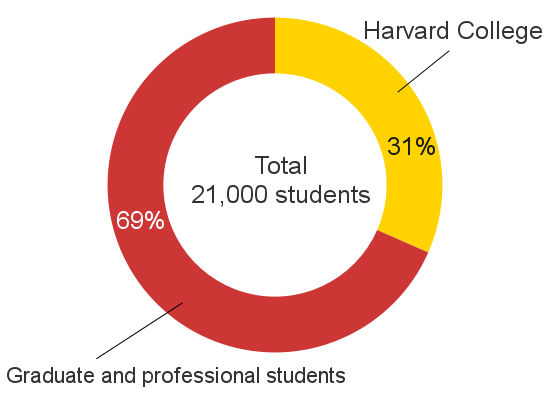
\includegraphics[width=0.3\textwidth]{images/fig1.png}

Harvard university include several universities, here is a list of the most important ones:\\
\begin{itemize}
  \item Faculty of Arts and Sciences composed by \\Harvard College \\Continuing Education \\Graduate School of Arts and Sciences \\Harvard John A. Paulson School of Engineering and Applied Sciences
\item Business School
\item Kennedy School of Government
\item Law School
\item Medical School
\item Radcliffe Institute
\item School of Education
\item Harvard T.H. Chan School of Public Health
\end{itemize}


\subsection{Harvard School of Engineering and Applied Sciences}
As you saw earlier ``beeing in Harvard'' without precising which university doesn't mean much, and so, during this in internship, I was affiliated to the Harvard School of Engineering and Applied Sciences, later called SEAS — Litte story: the school name changed during my journey, as Mr John A. Pauson did a donnation of \$ 400.000.000 to SEAS, so the school was rename after him.\\

The progenitor of the School of Engineering and Applied Sciences was called \textit{Lawrence Scientific School} and was founded in 1847. It was name for Abbott Lawrence, who donated \$50,000 (an unprecedented sum at the time) to create the institution. The was detached from Harvard College, which means it was independ financiery.
At this time, the School saw a diverse group of thinkers and professionals — astronomers, architects, naturalists, engineers, mathematicians, and even philosophers — pass through its doors.\\
At the end of the 19\textsuperscript{th} century, the school suffered the ``Competition'' from the new born Massachusset Institute of Technology (MIT) — Now one of the greatest engineering school in the world. The Harvard president of the time tried to merge the Harvard Scientific School with the MIT, vainly.\\
In 1901, despite the help of Gordon McKay, the school merged with Harvard College and lost his independance.\\

Later, the Harvard Lawrence Scientific School became \textit{The Division of Applied Science} and in 2007, it was rename as the \textit{Harvard School of Engineering and Applied Science}\\
It's a new start for the the School, Venkatesh Narayanamurti, Dean of Harvard School of Engineering and Applied Sciences at the time declared:\\
\say{\textit{Our transition from a Division to a School is not a departure from history—but in some sense, we are coming full circle. The Lawrence School, our progenitor, will be reborn in a new form appropriate for the 21st century.}}\\

Thus, strictly speaking, SEAS is a young school, only 8 years old, and in full growth. Thanks to the 4 milion dollars given by John Paulson, the school will expend and build laboratories in Allston, the city bordering Cambrigdge, on the other side of the river.\\

In order to realise the importance of Harvard engineering school in the world of sciences, here are a few examples of inventions made here:
\begin{itemize}
\item in 1919, the \textbf{crystal oscillator} came out of the Harvard Engineering School’s Cruft Laboratory, invented by George Washington Pierce
\item in 1938, the \textbf{largest cyclotron of the world} (at the time) was constructed at the Graduate School of Engineering's Gordon McKay Engineering Laboratory.
\item in 1977, Bill gates would have graduated from Harvard but he left the university  to found \textbf{Microsoft}, one of the biggest company in the world.
\item in 2004, \textbf{Facebook} was born in a dorm room of Harvard housing, created by Mark Zuckerberg, it's now the biggest social network ever created
\end{itemize}

\subsection{Mazur group}

\hseas{} is composed by several reseach groups. This summer, I worked with the group of professor Eric Mazur, Balkanski Professor of Physics and Applied Physics and Area Dean for Applied Physics.\\
Professor Mazur founded the group in 1111%I DON'T KNOW
to study the dynamics of molecules, chemical reactions, and condensed matter on very short timescales — down to femtoseconds ($10^{-15}$ second). Physics in this ultrafast regime is studied using light, specifically very short laser pulses. So the mazur group works with femtoseconds lasers.\\
In addition to the work in optical physics, The Mazur Group is very active in research about education. In 1990, Eric Mazur began developing Peer Instruction, a method for teaching large lecture classes interactively. He is the author of \textit{Peer Instruction: A User's Manual} (Prentice Hall, 1997), a book that explains how to teach large lecture classes interactively.

\newpage
\section{Organization}
\subsection{Main organization of the university}
Harvard University is huge. It's composed by a dozen of universities and it's under the direction of the president Drew Gilpin Faust and the provost Alan M. Garber.\\

Harvard is known to be a decentralized organization. Each constituent faculties has a lot of independence. This mean each faculties set their own academic standards and manage their own budgets. Each facultie is directed by the faculty dean whose role is to manage the matters of the facutly\\

Here you can see a chart representing the several faculties composing Harvard University (The one in which I worked is highlighted):\\
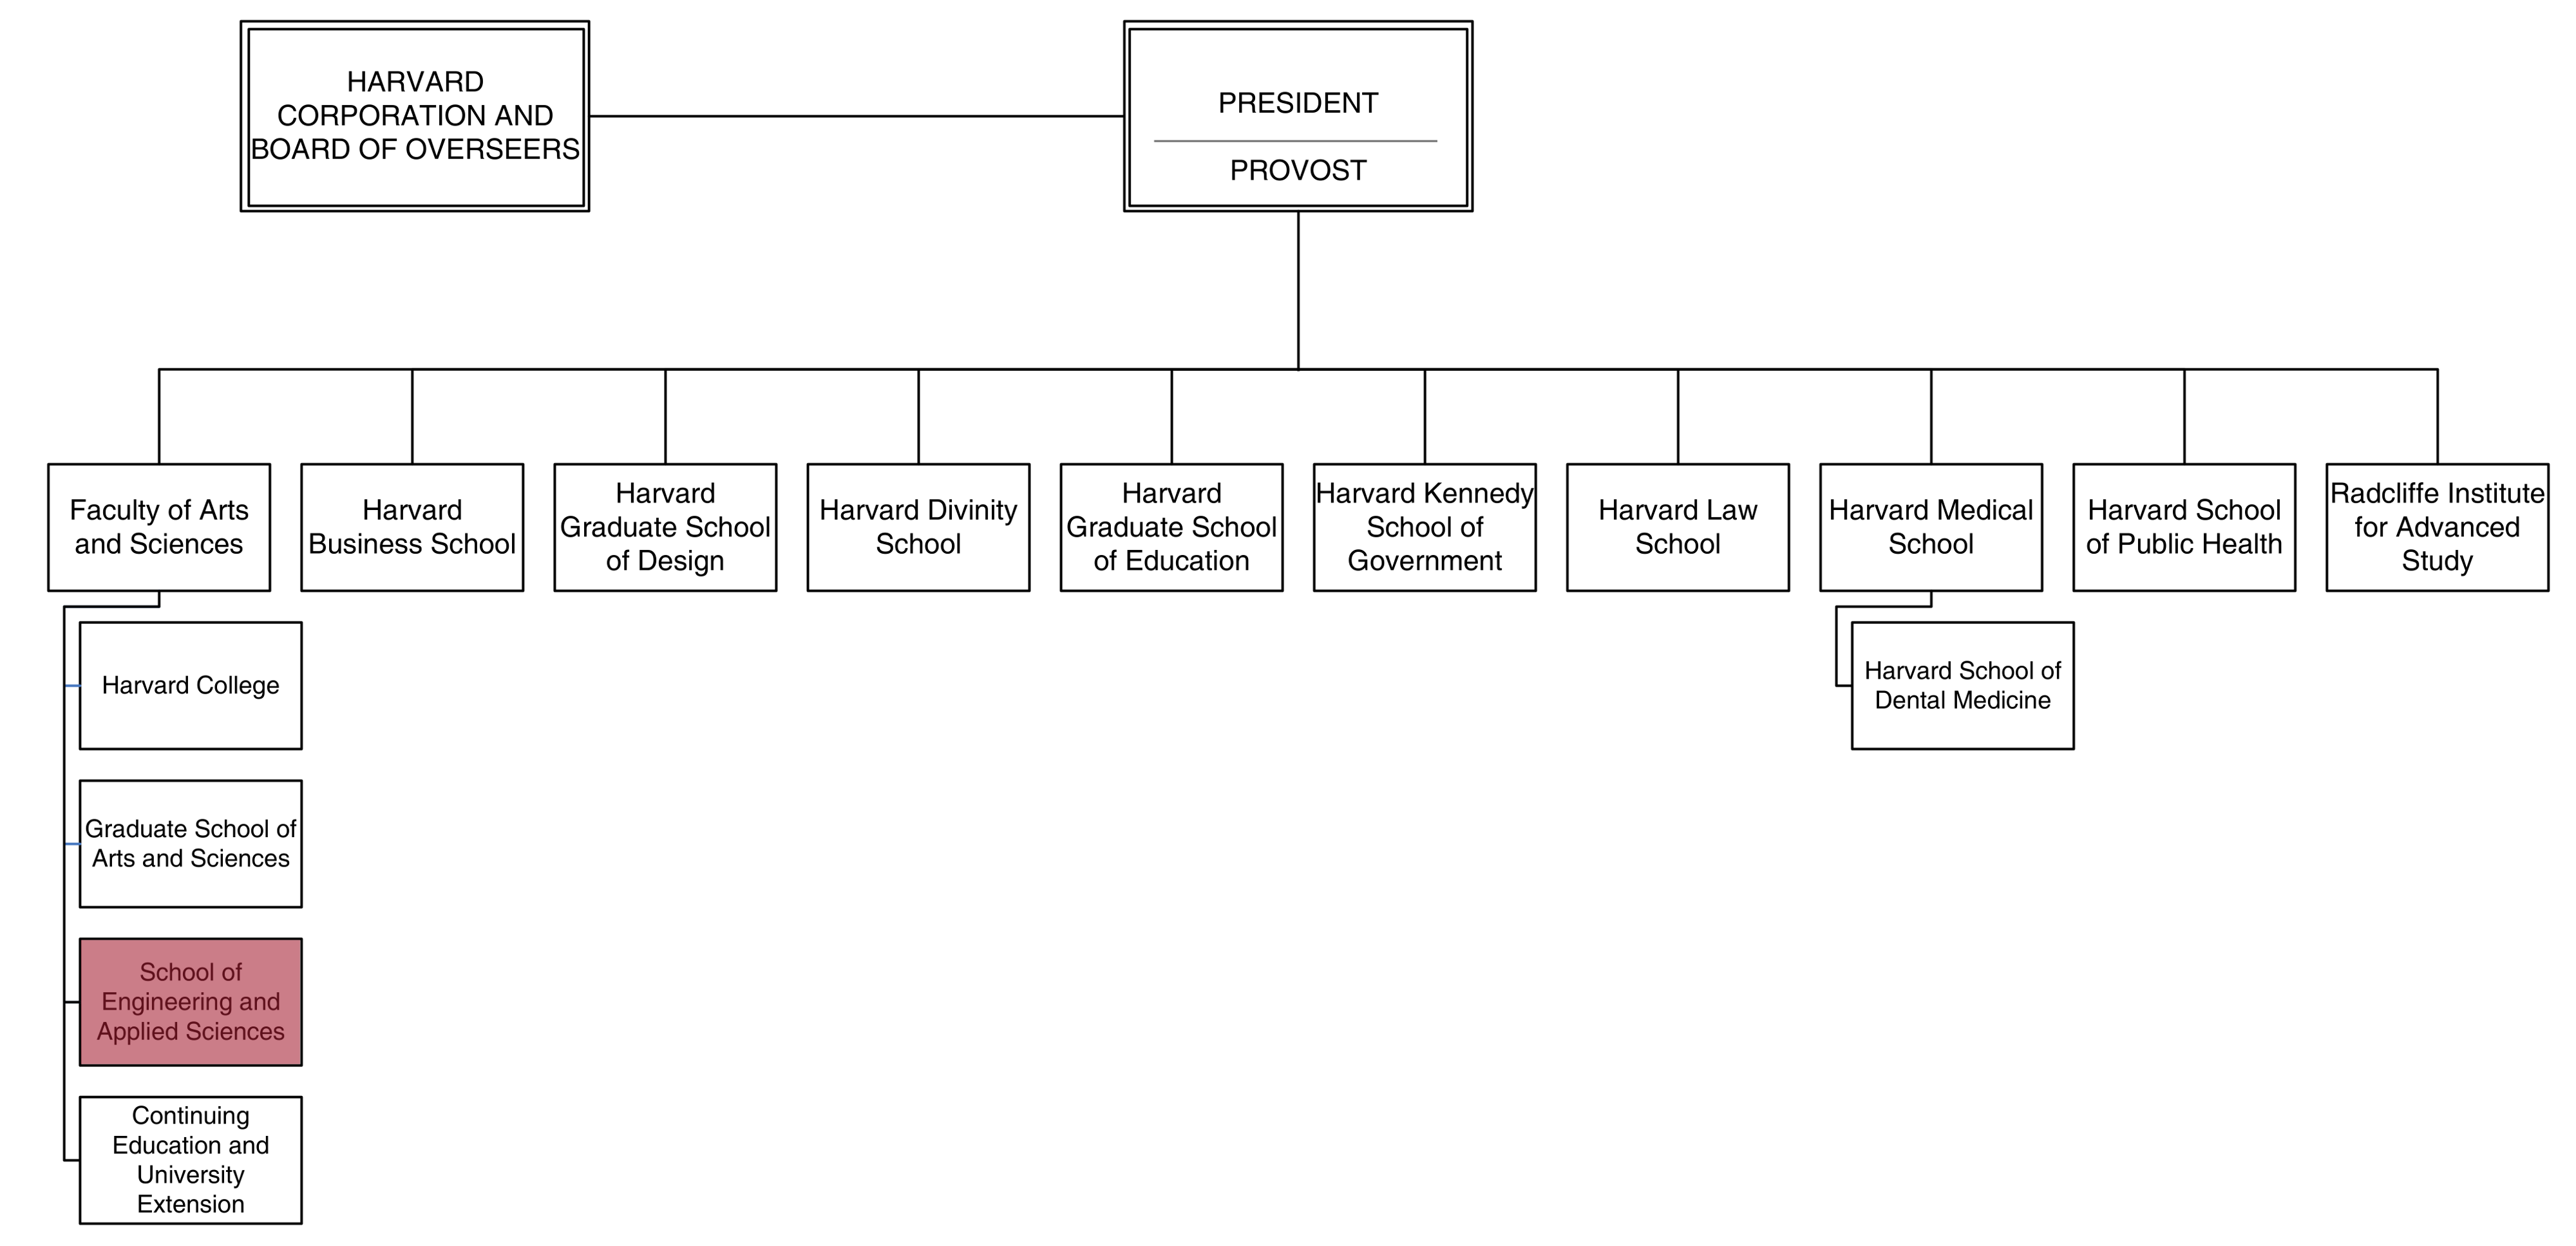
\includegraphics[width=1\textwidth]{images/chart1.png}

%Comment le président d'Harvard est il nommé ?
However, despite this decentralized management, the roles of the president and the provost are really important.\\

\textbf{The president} of Harvard university has two hats: Chief administrator of the university and the \textit{ex officio} chairman of the Harvard Corporation.
The president plays an important part in university-wide planning and strategy. She names a faculty's dean the university's provost, and she grants tenure to recommended professors. However, she is expected to make such decisions after extensive consultation with faculty members.\\
Moreover, as the leader of one of the most prominent universities in the world, Harvard presidents have influenced educational practices nationwide.\\

\textbf{The provost} of Harvard serves as chief academic officer. He works with the President to oversee academic policies and activities university-wide. The Office of the Provost works closely with the University’s academic and administrative leaders to: foster interfaculty collaboration, improve Harvard’s performance in building a diverse pipeline of scholars and in developing scholars at all stages of the academic career ladder, advance university-wide approaches to compliance and research policy, support University cultural and artistic entities and projects; oversee and coordinate the University’s international activities; support faculty, students, and academic professionals in advancing innovations in teaching and learning; and oversee activities pertaining to intellectual property, technology transfer, research collaborations with industry, and trademark licensing\footnote{provost.harvard.edu}.\\
%AS YOU CAN SEE _ON_ THIS CHART
The chart bellow represent the organization of the Harvard's central administration:\\
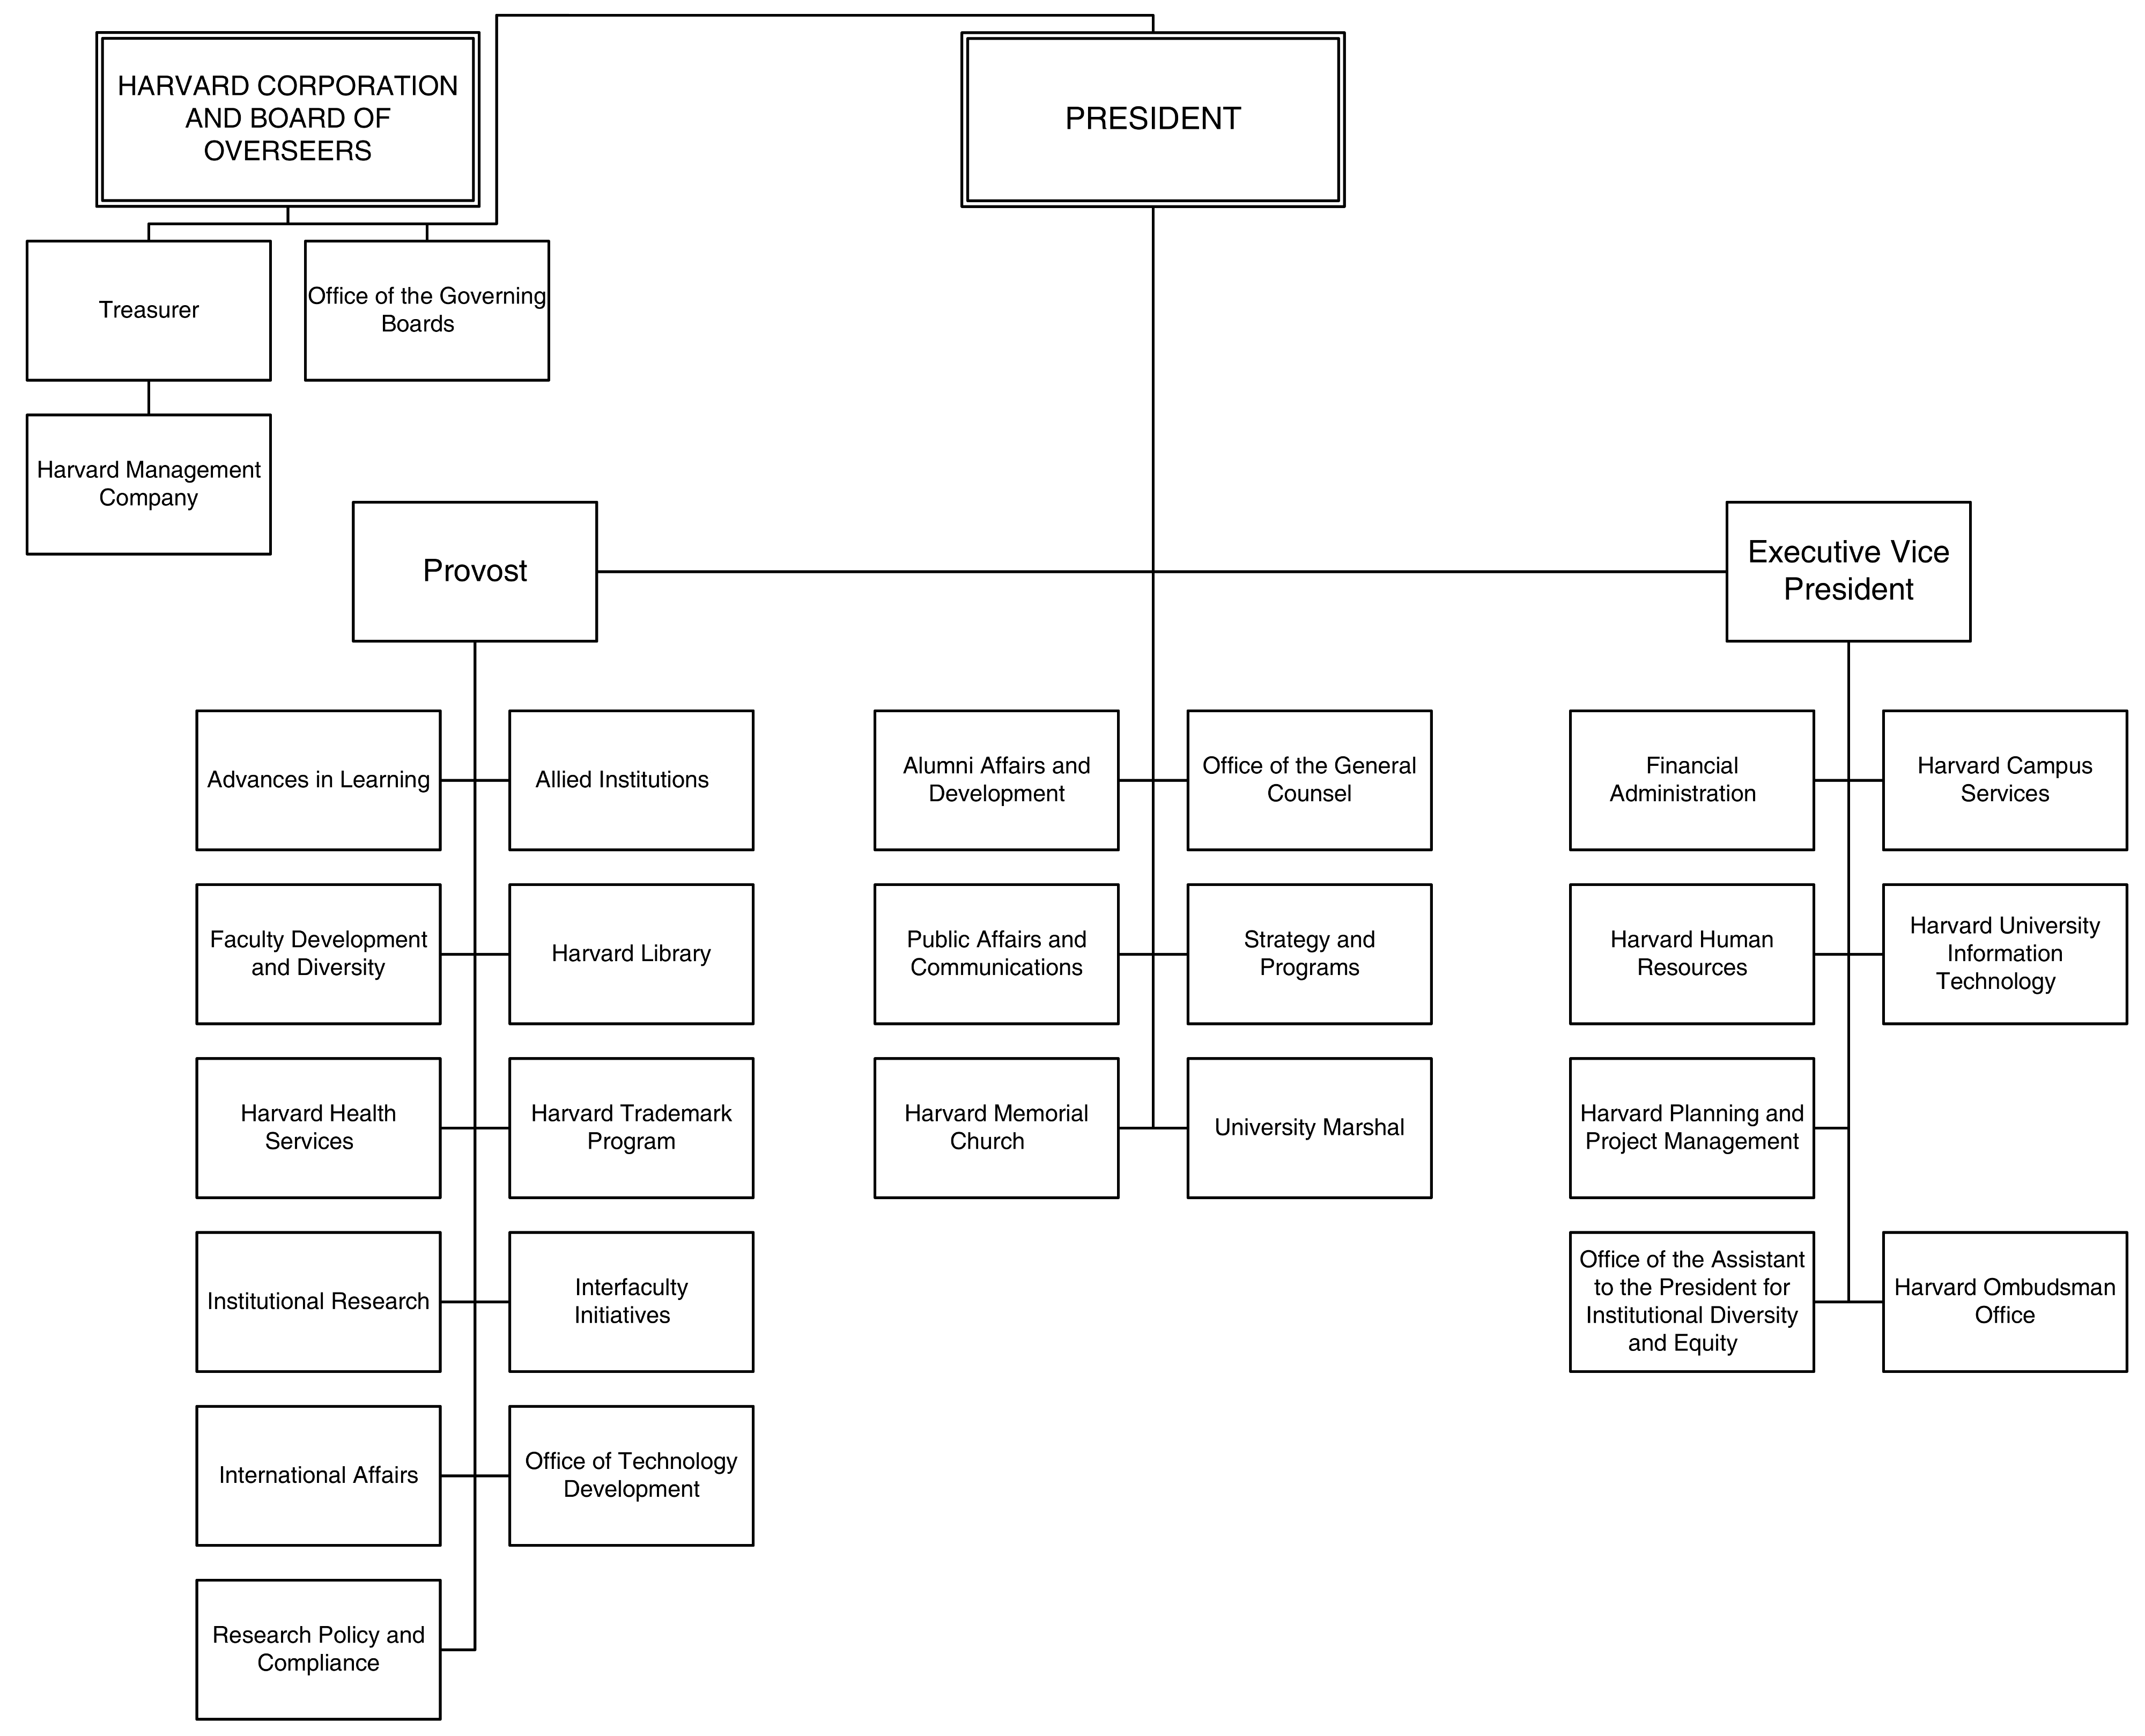
\includegraphics[width=1\textwidth]{images/chart2.png}
%TODO: COMMENT THIS CHART !

\subsection{Main organization of \hseas{}}
As I said earlier, each faculty composing Harvard university is very independent. As a consequence, \seas{} has it's own intern administration and financial management.\\
At the head of SEAS, we have the Dean, Francis J. Doyle III\@ His role is to manage new faculty recruitment and faculty relations, for example authorizing faculty searches, approving promotion reviews ans special appointments. Furthermore, he leads strategic planning for SEAS (mostly the financial needs) and he coordinates fundraising. He organizes the alumni relations, which are very important in a university such as Harvard.\\

The facutly is diveded into 8 ``areas'', at the head of which are the \textbf{area deans}.\\
Each area dean is helped in his work by the \textbf{area director}


%---------------------------------------
% PART II
%---------------------------------------
\newpage
\part{The internship}

\section{Mission and goals}
In the internship offer, my mission was described as following:\\

%------- QUOTE -----
\textit{We will update the Mazur group website. We need a student to port the php/mysql based Mazur group website to a new content management system and update photos and content.
Skills needed:
php/mysql experience required
experience with some content management platform (WordPress, drupal, etc.) preferred. Bonus points for Adobe suite or CSS template coding.}\\
%------- END QUOTE ---

I went on \textcolor{blue}{\underline{mazur.harvard.edu}} to see the website and I saw that it needed a wind of change. The design looks old and it doesn't fit to the screen, and the websites contains some dead links and not working search bars.\\
I was not sure yet about How will I work and I waited to see my mentor Daryl to have more infomation about the mission.\\

So, in my first day of internship, I met Daryl, a post-graduate student who work with the Mazur group, and she told me that a designer will take care of the \textbf{front-end } part. I was pretty happy with this news, since I don't master web design and it's not the part of web developpement I'm intersted in. Consequently, my job was to develop the \textbf{back-end} part of the website, i.e the PHP/SQL code which drives the core of the content management website. \\
Later, about a week after I started my internship, I met Eric Mazur, principal investigator of the group, he gave me his specifications.

\subsection{Specifications}
Basically the goal of my mission was to create a new website for the Mazur group, whith pretty much the same features as the old one which are in a nutshell:
\begin{itemize}
\item For the visitor: Navigate through the contents (Publications, Talks, People, News about the group)
\item Be able to search overall the website
\item For the members of the group: Add, update and delete content.
\end{itemize}

\subsection{Difficulties encoutered}
%OLD CODE AND DATABASE

\subsubsection*{Languages and technologies}
When I started to work on the website, my first task was to download the old website and database on my computer so I could work locally without ``damaging'' the current website.\\

I discovered that the database management system was \textbf{PostgreSQL}. I have always worked with \textbf{MySQL} as a management system and so I wasn't familliar at all with Postgre.\\
So, one of my first task during this internship was to install a PotgreSQL server on my computer which runs on ubuntu, simply by executing \shellcmd{sudo apt-get install postgresql} in the terminal.\\
Then, once I had installed the server locally, I nedded to import the current database and learn how to use Posgresql. I used a lot the documentation on PostgreSQL offical website\footnote{www.postgresql.org} which is really complete.\\

For a little while, I navigated through the database using command line, but it wasn't practical at all. Thus, I looked for a graphical user interface administration tool for managing the database, an equivalent of phpMyAdmin but for PostgreSQL, which would help me to manage the database.\\
I chose to install \textit{PgAdminIII}, a powerful tool that allows me to manage the database, see the tables, execute queries\ldots
%A VOIR: METRE UN SCREENSHOT DU SOFT ??

In conclusion, learning how to use PostgreSQL wasn't so hard but it took me about a whole week to be really used to it. The query syntax is SQL so it wasn't different from I learnt at school.

\subsubsection*{Database}
Once I mastered PostgreSQL and database management, I started to look at the current database organization of the website. The fist thing I noticed was that it was very disordered. The database contained 196 tables where about a hundred was empty. Moreover, the encoding of the data was ASCII, a very old encoding format which can represent only 128 characters.\\
Thus, the first thing I did with the database was to convert it into UTF-8 encoding, a modern character encoding system, compatible with ASCII and way more complete.\\ Thanks to that, special characters such as ``é'' or ``ï'' can now be used in the database.\\

After looking at all the tables in the database, I decided to create a new one, and import tables that I wanted in it, so that this database would be ``cleaner''. In order to easily transfer tables from a database to the other, I wrote a shell script which automatize the process:\\

\begin{lstlisting}[language=bash]
#!/bin/bash
#Transfers tables from old database to new one
pg_dump -h localhost -U mazur_www mazur_www_utf8 --table $1 > /tmp/$1.pgsql #Exporting
psql -h localhost -U mazur_www mazur_db < /tmp/$1.pgsql #Importing
rm /tmp/$1.pgsql #Cleaning
\end{lstlisting}

In order to understand the database main organization, I tried to build a little UML diagram, which I expanded throughout the internship. I used the website yuml.com%aferifer
to


\subsubsection*{Independance}
During this internship, I had a really great independance. I worked mostly with the IT-Team of \hseas{} so I could ask them if had questions, but my internship master wasn't there most of the time. It was


\section{Work organization}
As I said earlier, I was very indepandant during this internship, I had to manage myself. My mission was to create a website but it was up to me to organise my schedule and my short terms objectives.\\
In order to keep organised, I always had a little notebook next to my laptop when I worked, on which I wrote my short terms objectives. It was mostly organized as TODO lists, comporting a few tasks that I tried to do as soon as I could.\\
I also used this notebook as a rough book to draw UML diagram, graphic SQL queries or pseudo-code for algorithms.\\

It was really hard to manage the work by myself and it took me a while to be really organized. At the begining, %TODO: CONTINUE !

\subsection{Tools}

During the whole internship, the only hardware that I used was my own computer. I prefered work on this one instead of a Harvard's one because I'm used to it and there is an AZERTY keyboard and that makes a big difference.\\
My computer is a \textit{HP Pavillon 15n} running on Ubuntu Linux 14.04. It has an Intel Core i5 CPU and 8 Go of RAM\@. this configuration is quite sufficient to do web development.\\

No complicated or expensive softwares are needed to develop a website. The main languages I used were PHP, mySQL and Javascript. These languages don't need any compilation and a simple notepad application could suit for web developement. Nontheless, I started my internshipt using Sublime Text to code, this software is an ``improved'' nodepad, with some features such as autocompletion, autoindent, bracket-matching \ldots \\
About a month after I stared my internship, I asked my coworkers from the IT-team which software they used for web developpement and which one they would recomand. A coworker told me that he developed on a paid (and expensive) software, but he recomanded me \textit{Atom}, an open source free software pretty close to Sublime Text. I tried this software and I immediatly adopted it.\\
The functionment of Atom is simple, it's a the beginning a simple notepad application but you can add packages for autocompletion, spell-checking, linting\ldots \\
So I developped the entire website using Sublime Text, then Atom.


Of course I needed a web browser to visualise and test the website. I chose Mozilla Firefox, my usual web browser, it's open source and it come with a lot of usefull ``developper tools'' really usefull when you want to test a website. For example:
\begin{itemize}
\item I could edit CSS code directly while navigating on the webpage.
\item I used the javascript console to see errors and to inject code into the webpage in order to test my code.
\item Theses tools allowed me to inspect the network, so I could see the HTTP requests done by the website.
\item I could also monitor the loading time of a webpage, and optimize it by improving and compressing my javascript code for example.
\item The website needs to be adapted for a smatphone browsing, Firefox offers the possibility to simulate the behaviour of a smartphone with the ``adaptive view''.
\end{itemize}

Nevertheless, I also needed to test my website on other web browser, in order to be sure that everything is working. So thanks to VMWare player I could launch a windows 7 and a MacOS X Yosemete to see the behaviour of the website on Internet Explorer and Safari.

\section{Skills used}

I started to interest myself in website creation when I was in high school. I was very curious about how a website is made, how is it hosted\ldots So, I learned the basics of website creation when I was 17, using the famous MOOC\footnote{Massive Open Online Course, a website which aims to provide open courses online} \textit{Le site du zéro}, now called \textit{Openclassrom}.\\
I learned HTML/CSS and php and I had a some knowledge in SQL. I didn't know anything about javascript.
Then, when I came to ECE Paris Engineering School, I learnt the theory behind SQL and database management. These courses and the JAVA project \textit{Gestion d'un centre hospitalier} has been very usefull for me during this internship which involved a lot of databasing.\\
Morever, this year I worked on a \textbf{Projet pluridiciplinaire en équipe} whithin the ECE and I had to developp a web interface using javascript and a Node.js server, also using javascript. All my javascript/jQuery knowledge come from this project, and it has been a tremendous help during this summer.\\

The other kind of skills that I used a lot is Linux management and shell script.\\
The communication beetween my computer and Havard server was via \textbf{ssh}. As Linux has a native ssh client included it was pretty easy.\\
Then, as you saw earlier, I wrote some \textbf{shell scripts} to avoid typing the same commands again and again. The courses of Laurent Ferrier about Linux taught me how to write shell script.


\section{Results}










\end{document}
